\newpage
\section{2023秋}

\setcounter{yearcounter}{2023}
% \setcounter{page}{1}

\subsection{微分積分}
\prob{%
  次のように\dm{x,y}が変数\dm{t}の関数として与えられるとき,
  \dm{x,y}を用いて\dm{\frac{dy}{dx}}を表せ。
  \al{
    \begin{dcases*}
      x = \frac{2t}{t^2 + 1} \\
      y = \frac{t^2 - 1}{t^2 + 1} \\
    \end{dcases*}
  }
}
\begin{ans*}
  与式より$x^2 + y^2 = 1$であるので両辺を$x$で微分して
  \begin{gather}
    2x + 2y\frac{dy}{dx} = 0 \\
    \frac{dy}{dx} = -\frac{x}{y}
  \end{gather}
\end{ans*}
\prob{%
  以下の問いに答えよ。
  \begin{enumerate}[label=(\arabic*)]
    \item 次に示す関数\dm{f(t)}および\dm{g(t)}を\dm{t=0}のまわりでそれぞれテイラー展開せよ。
    \al{f(t) = \sin t,\quad g(t) = \cos t}
    \item 次に示す2次の正方行列\dm{\bA}と単位行列\dm{\bE}を考える。
    \dm{n}をゼロ以上の整数とし,\dm{n,t,\bE}を用いて\dm{\bA^2}および
    \dm{\bA^{2n}}を表せ。なお,\dm{\bA^0}は\dm{\bE}と定義される。
    \al{
      \bA =
      \begin{pmatrix}
        0 & -t \\
        t & 0
      \end{pmatrix}
      ,\quad
      \bE = 
      \begin{pmatrix}
        1 & 0 \\
        0 & 1 
      \end{pmatrix}
    }
    \item 行列\dm{\bA}の指数関数\dm{\exp \bA}は次のように定義される。
    \dm{\sin t}と\dm{\cos t}を用いて\dm{\exp \bA}のすべての成分を表せ。
    \al{\exp\bA = \sum_{k=0}^{\infty}\frac{1}{k!}\bA^k = \bE + \frac{1}{1!}\bA + \frac{1}{2!}\bA^2 + \cdots}
  \end{enumerate}
}
\begin{ans*}
  ${}$
  \begin{enumerate}[label=(\arabic*)]
    \item テイラー展開はそれぞれ
    \begin{align}
      f(t) 
      &= \sum_{n=0}^{\infty} \frac{f^{(n)}(0)}{n!} t^n \\
      &= t - \frac{t^3}{3!} + \frac{t^5}{5!} - \frac{t^7}{7!} + \cdots \\
      g(t)
      &= 1 - \frac{t^2}{2!} + \frac{t^4}{4!} - \frac{t^6}{6!} + \cdots
    \end{align}
    \item 与えられた行列について,$\bA^2$は
    \begin{align}
      \bA^2
      &=
      \begin{pmatrix}
        0 & -t \\
        t & 0 
      \end{pmatrix}
      \begin{pmatrix}
        0 & -t \\
        t & 0
      \end{pmatrix} \\
      &= -t^2
      \begin{pmatrix}
        1 & 0 \\
        0 & 1
      \end{pmatrix} \\
      &= -t^2 \bE
    \end{align}
    また,$\bA^{2n}$は
    \begin{align}
      \bA^{2n}
      &=
      \begin{dcases*}
        (-t^{2})^{n}\bE & if $n\geq 1$ \\
        \bE & if $n = 0$
      \end{dcases*} \\
      &= (-t^{2})^{n}\bE    
    \end{align}
    \item (2)より
    \begin{align}
      \exp\bA
      &= 
      \bE + \frac{1}{2!}\bA^2 + \frac{1}{4!}\bA^4 + \frac{1}{6!}\bA^6 + \cdots 
      + \frac{1}{1!}\bA + \frac{1}{3!}\bA^3 + \frac{1}{5!}\bA^5 + \cdots \\
      &= 
      \bE - \frac{t^2}{2!}\bE + \frac{t^4}{4!}\bE - \frac{t^6}{6!}\bE + \cdots 
      + \frac{1}{1!}\bA - \frac{t^2}{3!}\bA + \frac{t^4}{5!}\bA - \cdots \\
      &=
      \bE - \frac{t^2}{2!}\bE + \frac{t^4}{4!}\bE - \frac{t^6}{6!}\bE + \cdots 
      + \frac{1}{1!}\bA - \frac{t^2}{3!}\bA + \frac{t^4}{5!}\bA - \cdots \\
      &=
      \Bigl(1 - \frac{t^2}{2!} + \frac{t^4}{4!} - \frac{t^6}{6!} + \cdots \Bigr)\bE 
      + \Bigl(\frac{t}{1!} - \frac{t^3}{3!} + \frac{t^5}{5!} - \cdots \Bigr)
      \begin{pmatrix}
        0 & -1 \\
        1 & 0
      \end{pmatrix} \\
      &=
      \cos t
      \begin{pmatrix}
        1 & 0 \\
        0 & 1 
      \end{pmatrix}
      +
      \sin t
      \begin{pmatrix}
        0 & -1 \\
        1 & 0 
      \end{pmatrix} \\
      &=
      \begin{pmatrix}
        \cos t & -\sin t \\
        \sin t & \cos t 
      \end{pmatrix}
    \end{align}
    
  \end{enumerate}
  
\end{ans*}

\prob{%
  次の重積分について,以下の問いに答えよ。
  \al{
    I = \iint_D x \:dx dy,\quad D = \left\{(x,y)\relmiddle x\geq 0, y\geq 0, 1\leq x^2 + y^2\leq 2y\right\}
    }
  
  \begin{enumerate}[label=(\arabic*)]
    \item 積分領域\dm{D}を図示せよ。
    \item 重積分\dm{I}を計算せよ。
  \end{enumerate}
}
\begin{ans*}
  ${}$
  \begin{enumerate}[label=(\arabic*)]
    \item 積分領域\dm{D}は下図
    
    \begin{figure}[H]\centering
      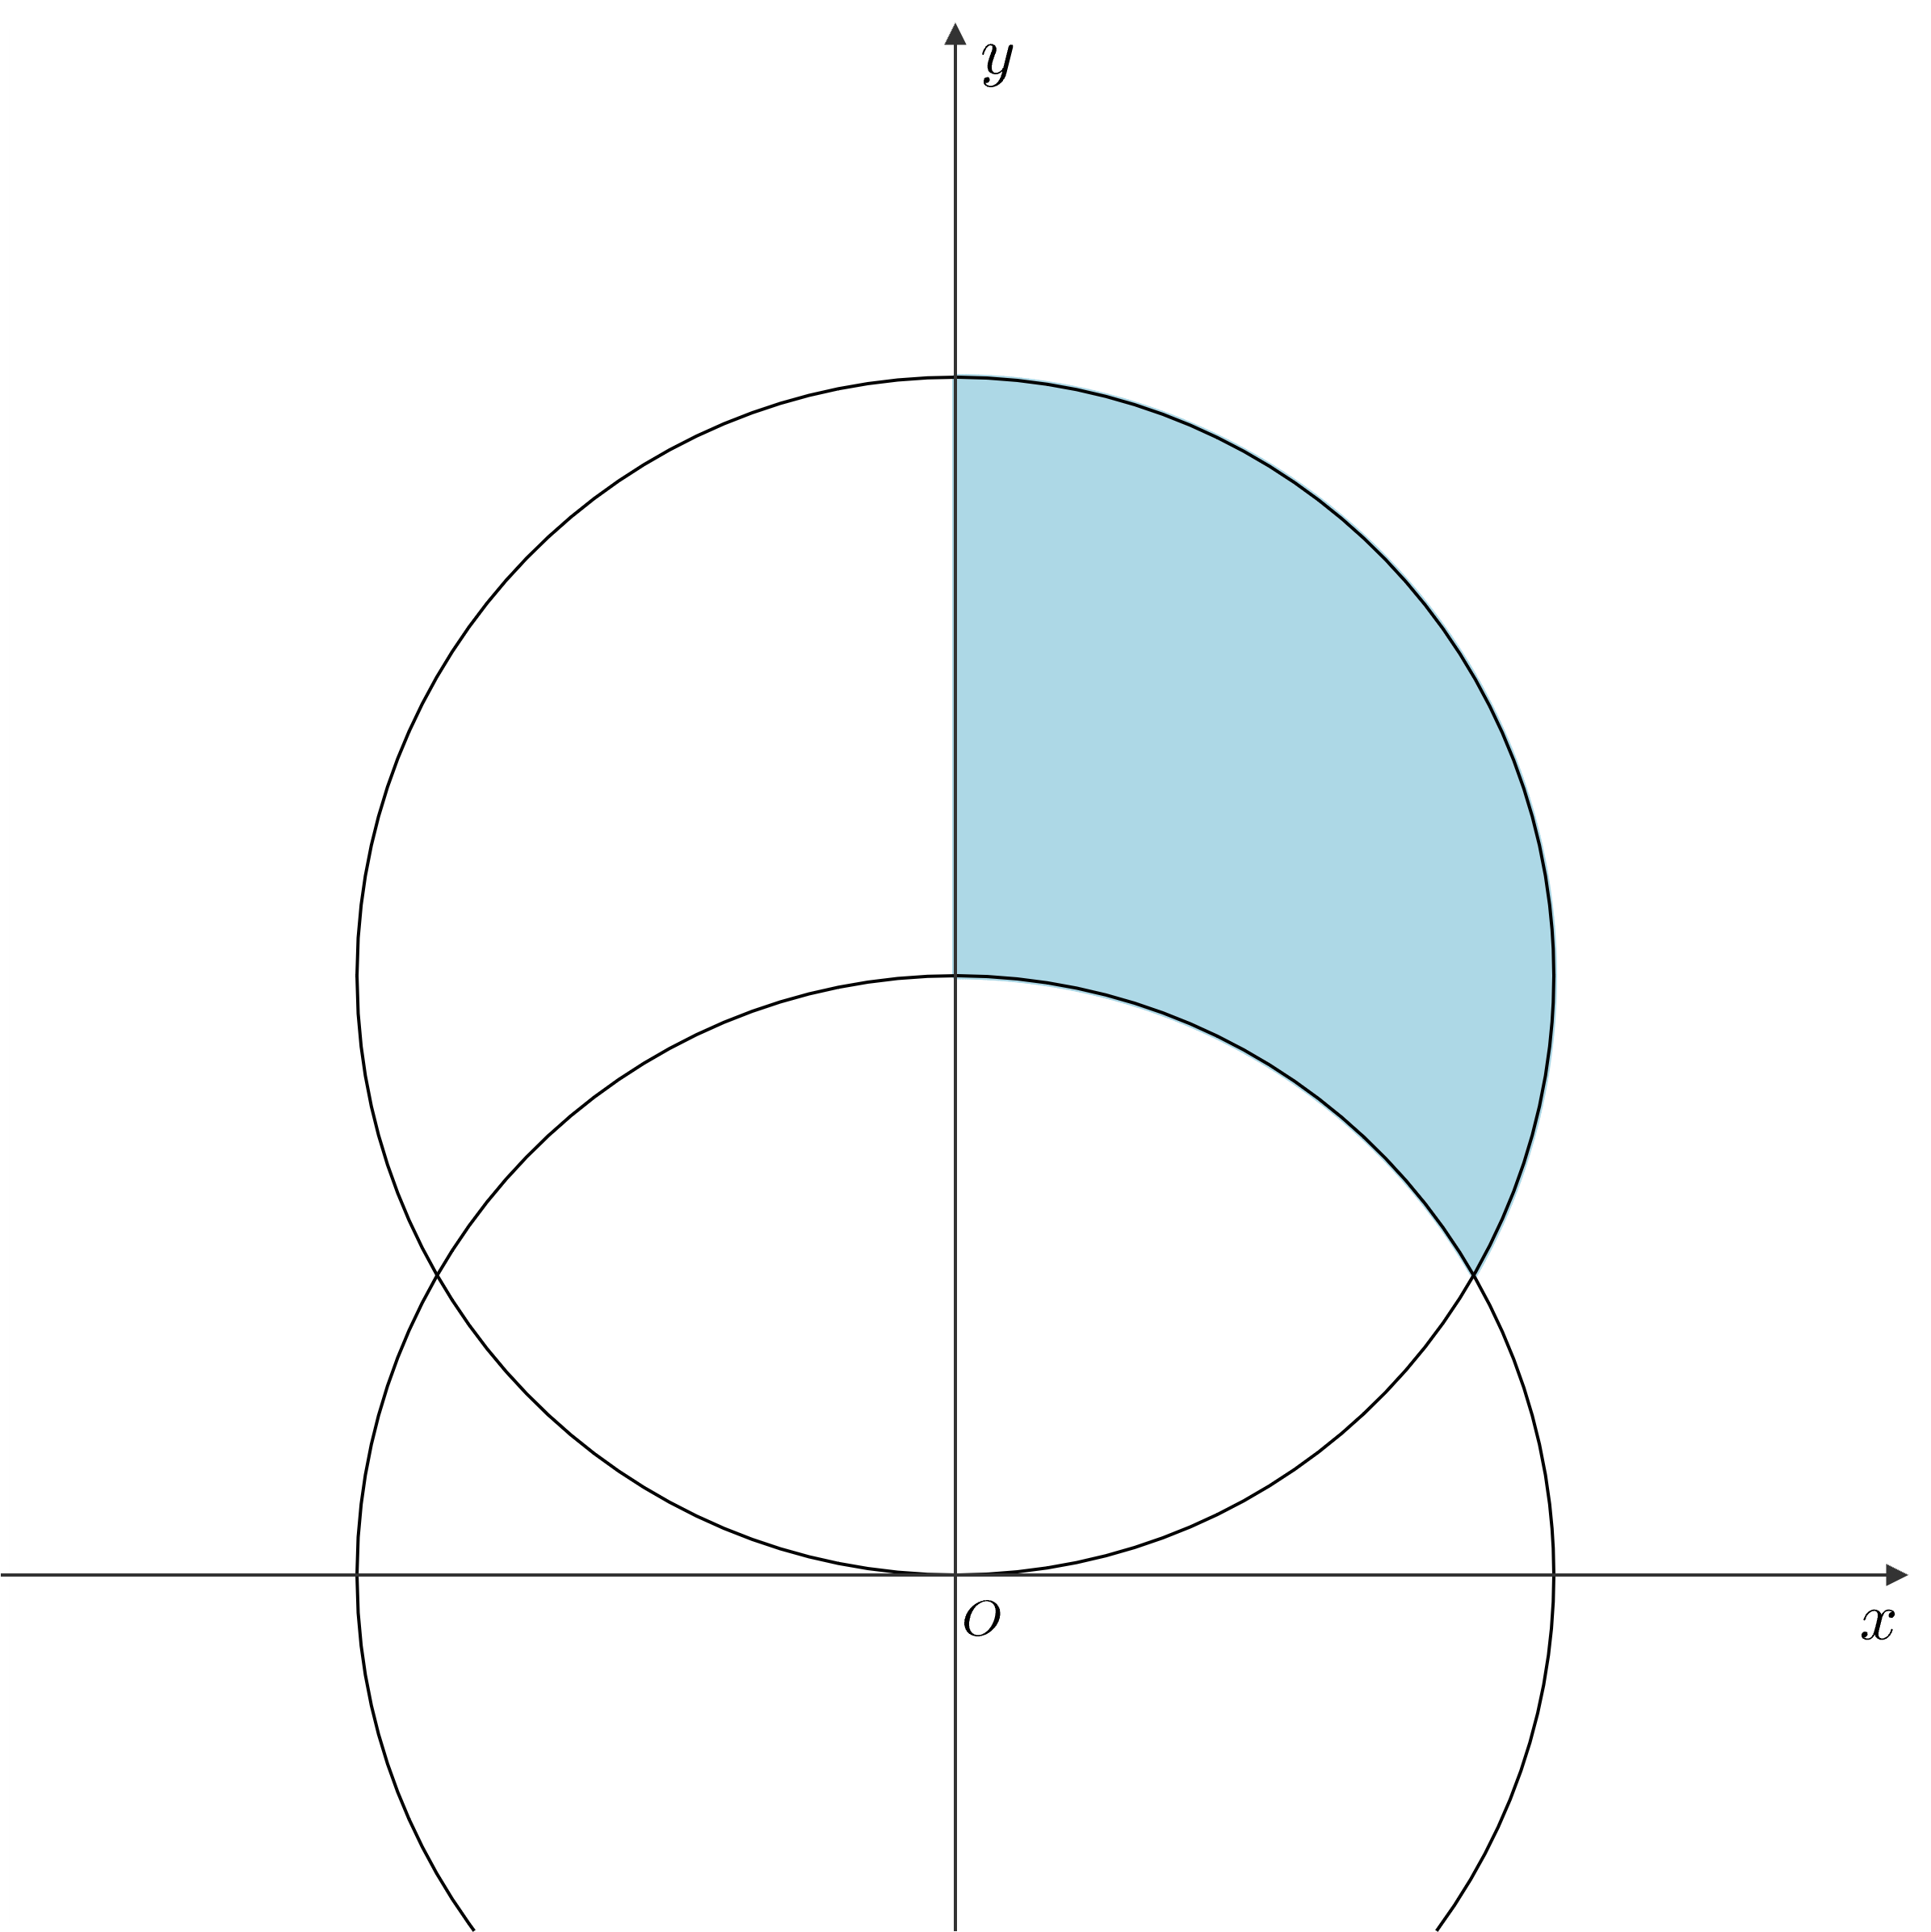
\includegraphics[width=.5\linewidth]{./src/asset/fig/2023_D.png}
    \end{figure}
    
    \item 
    与えられた積分について極座標変換\dm{x = r\cos\theta,y=r\sin\theta}を考えると,
    領域\dm{D}は
    \al{
      D &= \left\{(r,\theta)\relmiddle r\geq 0, 0\leq\theta\leq\frac{\pi}{2}, 1\leq r^2 \leq 2r\sin\theta\right\}\\
        &= \left\{(r,\theta)\relmiddle r\geq 0, 0\leq\theta\leq\frac{\pi}{2}, 1\leq r \leq 2\sin\theta\right\}\\
        &= \left\{(r,\theta)\relmiddle 0\leq\theta\leq\frac{\pi}{2}, 1\leq r \leq 2\sin\theta\right\}\\
        &= \left\{(r,\theta) \relmiddle \frac{\pi}{6}\leq\theta\leq\frac{\pi}{2}, 1\leq r \leq 2\sin\theta\right\}\quad(\because 1\leq 2\sin\theta)
    }
    である。\dm{dxdy = r\:drd\theta}も考えて,
    \al{
      I
      &= \int_{\pi/6}^{\pi/2}\int_{1}^{2\sin\theta} r^2\cos\theta \:drd\theta  \\
      &= \int_{\pi/6}^{\pi/2}d\theta \left[ \frac{r^3}{3}\cos\theta \right]_{1}^{2\sin\theta} \\
      &= \int_{\pi/6}^{\pi/2}\left( \frac{8}{3}\sin^3\theta\cos\theta - \frac{1}{3}\cos\theta \right) \:d\theta \\
      &= \frac{1}{3}\int_{1/2}^{1}(8t^3-1) \:dt \\
      &= \frac{1}{3}\left[ 2t^4 - t \right]_{1/2}^{1} \\
      &= \frac{11}{24}
    }
  \end{enumerate}
  \begin{other*}
    領域\dm{D}は
    \al{
      D
      &= \left\{(x,y)\relmiddle x\geq 0, y\geq 0, 1\leq x^2 + y^2\leq 2y\right\} \\
      \begin{split}
        &= \left\{(x,y)\relmiddle 0\leq x\leq \frac{\sqrt{3}}{2}, \sqrt{1-x^2}\leq y\leq \sqrt{1-x^2}+1 \right\} \\
        &\hspace*{50pt} \vee \left\{(x,y)\relmiddle \frac{\sqrt{3}}{2}\leq x\leq 1, -\sqrt{1-x^2}+1\leq y\leq \sqrt{1-x^2}+1 \right\}
      \end{split}
    }
    とも表せるので,重積分\dm{I}は
    \al{
      I
      &= \int_{0}^{\sqrt{3}/2}\int_{\sqrt{1-x^2}}^{\sqrt{1-x^2}+1} x\:dydx
         + \int_{\sqrt{3}}^{1}\int_{-\sqrt{1-x^2}+1}^{\sqrt{1-x^2}+1}x\:dydx \\
      &= \int_{0}^{\sqrt{3}/2} x \:dx + \int_{\sqrt{3}/2}^{1}2x\sqrt{1-x^2}\:dx \\
      &= \left[\frac{1}{2}x^2\right]_{0}^{\sqrt{3}/2} + \int_{3/4}^{1}\sqrt{1-t}\:dt \quad(t=x^2) \\
      &= \frac{1}{2}\cdot\frac{3}{4} + \left[-\frac{2}{3}(1-t)^{3/2}\right]_{3/4}^{1} \\
      &= \frac{11}{24}
    }
  \end{other*}
\end{ans*}





%@ =========================================================
%@ =========================================================
%@ =========================================================
\subsection{線形代数}
\prob{%
  ベクトル\dm{\ba}および\dm{\bb}に関する以下の問いに答えよ。
  \al{
    \ba = 
    \begin{pmatrix}
      \:\: 1 \:\:\:\\ 2 \\ 1
    \end{pmatrix}
    ,\quad
    \bb = 
    \begin{pmatrix}
    \:\:  -4 \:\:\:\\ 11 \\ 6
    \end{pmatrix}
  }
  \begin{enumerate}[label=(\arabic*)]
    \item ベクトル\dm{\bb}を,\dm{\ba}を通る直線へ射影せよ。
    \item \dm{\ba}を通る直線への射影行列\dm{\bm{P}}を求めよ。
  \end{enumerate}
}
% []: 射影の説明
\begin{ans*}
  ${}$
  \begin{enumerate}[label=(\arabic*)]
    \item ベクトル\bb の\ba への射影\bm{p}は\dm{\bm{p} = \frac{\ba}{|\ba|}|\bb|\cos\theta}より
    \begin{align}
      \bm{p}=\mathrm{proj}_{\ba} \bb
      = \frac{\ba\cdot\bb}{|\ba|^2}\:\ba
      =
      4
      \begin{pmatrix}
      \:\:  1 \:\:\:\\ 2 \\ 1 \\
      \end{pmatrix}
    \end{align}
    \item \dm{\bm{P} = \frac{\ba\ba^T}{\ba^T\ba}}は
    \begin{align}
      \bm{P}
      = \frac{1}{6}
      \begin{bmatrix}
        1 & 2 & 1 \\ 2 & 4 & 2 \\ 1 & 2 & 1
      \end{bmatrix}
    \end{align}
    % あるいは
    % \begin{align}
    %   \bm{p} = \bm{P}\bb
    % \end{align}
    % から
  \end{enumerate}
\end{ans*}

\prob{%
  \dm{\bA = \bL\bU}とする下三角行列\dm{\bL}と上三角行列\dm{\bU}を求めよ。
  ただし,下三角行列\dm{\bL}の対角成分は1とする。
  \al{
    \bA = 
    \begin{pmatrix}
      a & a & a \\
      a & b & b \\
      a & b & c 
    \end{pmatrix}
  }
}
\begin{ans*}
  行列\dm{\bL,\bU}の未知の\dm{i}行\dm{j}列の要素を
  \dm{l_{ij},u_{ij}}と表すとき,
  \dm{\bL\bU}分解は
  \al{
    \bA 
    &=   
    \bL\bU \\
    &= 
    \begin{pmatrix}
      1 & 0 & 0 \\
      l_{21} & 1 & 0 \\
      l_{31} & l_{32} & 1 \\
    \end{pmatrix}
    \begin{pmatrix}
      u_{11} & u_{12} & u_{13} \\
      0 & u_{22} & u_{23} \\
      0 & 0 & u_{33} \\
    \end{pmatrix} \\
    &=
    \begin{pmatrix}
      u_{11} & u_{12} & u_{13} \\
      l_{21}u_{11} & l_{21}u_{12}+u_{22} & l_{21}u_{13}+u_{23} \\
      l_{31}u_{11} & l_{31}u_{12}+l_{32}u_{22} & l_{31}u_{13}+l_{32}u_{23}+u_{33} \\
    \end{pmatrix}
  }
  とできるので,
  \begin{gather}
    \bL = 
    \begin{pmatrix}
      1& 0& 0 \\
      1& 1& 0 \\
      1& 1& 1 \\
    \end{pmatrix} \\
    \bU =
    \begin{pmatrix}
      a& a& a \\
      0& b-a& b-a \\
      0& 0& c-b \\
    \end{pmatrix}
  \end{gather}
\end{ans*}

\prob{%
  行列\dm{\bB}に関する以下の問いに答えよ。
  \al{\bB = 
    \begin{pmatrix}
      {\displaystyle \frac{5}{6}} & {\displaystyle \frac{1}{3}} \\
      \\
      {\displaystyle \frac{1}{6}} & {\displaystyle \frac{2}{3}} \\
    \end{pmatrix}
  }
  \begin{enumerate}[label=(\arabic*)]
    \item \dm{\bB}の固有値をすべて求めよ。
    \item \dm{\bB^2}の固有値をすべて求めよ。
    \item \dm{\bB^{\infty}}を求めよ。
  \end{enumerate}
}
\begin{ans*}
  ${}$
  \begin{enumerate}[label=(\arabic*)]
    \item \bB の固有方程式\dm{\det(\bB-\lambda\bE)=0}より
    \al{
      \det(\bB-\lambda\bE) 
      &= 
      \Bigl(\lambda-\frac{5}{6}\Bigr)\Bigl(\lambda-\frac{2}{3}\Bigr)-\frac{1}{18} \\
      &= \frac{1}{2}(\lambda - 1)(2\lambda - 1) \\
      &\therefore \lambda = \frac{1}{2}, 1
    }
    \item 
    \dm{\bB^2}は
    \begin{gather}
      \bB^2 = 
      \begin{pmatrix}
        {\disp \frac{3}{4}} & {\disp \frac{1}{2}} \\
        \\
        {\disp \frac{1}{4}} & {\disp \frac{1}{2}} \\
      \end{pmatrix}
    \end{gather}
    であるので,\dm{\bB^2} の固有方程式\dm{\det(\bB^2-\lambda\bE)=0}より
    \al{
      \det(\bB^2-\lambda\bE) 
      &= 
      \Bigl(\lambda-\frac{3}{4}\Bigr)\Bigl(\lambda-\frac{1}{2}\Bigr)-\frac{1}{8} \\
      &= \frac{1}{4}(\lambda - 1)(4\lambda - 1) \\
      &\therefore \lambda = \frac{1}{4}, 1
      }

    \item 
    \bB は対角化行列\bP を用いて
    \begin{gather}
      \bP^{-1}\bB\bP = 
      \begin{pmatrix}
        {\disp \frac{1}{2}} & 0 \\
        \\
        0 & {1} \\  
      \end{pmatrix}
    \end{gather}
    と対角化される。このとき対角化行列\bP について
    
    \begin{enumerate}[label=(\roman*)]
      \item \dm{\lambda = \frac{1}{2}}のとき
      \begin{gather}
        (\bB -\lambda\bE)\bu = \bm{0} \\
        \bu = \begin{pmatrix} x \\ y \end{pmatrix} \\
        \Rightarrow
        \begin{pmatrix}
          {\disp\frac{1}{3}} & {\disp\frac{1}{3}} \\&\\ {\disp\frac{1}{6}} & {\disp\frac{1}{6}}
        \end{pmatrix}
        \begin{pmatrix}
          x \\ y
        \end{pmatrix}
        =\bm{0}
      \end{gather}
      であるので,固有ベクトルは
      \begin{gather}
        \bu = 
        \begin{pmatrix}
          1 \\ -1
        \end{pmatrix}
      \end{gather}
      \item \dm{\lambda = 1}のとき
      \begin{gather}
        (\bB -\lambda\bE)\bu = \bm{0} \\
        \bu = \begin{pmatrix} x \\ y \end{pmatrix} \\
        \Rightarrow
        \begin{pmatrix}
          {\disp -\frac{1}{6}} & {\disp\frac{1}{3}} \\&\\ {\disp\frac{1}{6}} & {\disp -\frac{1}{3}}
        \end{pmatrix}
        \begin{pmatrix}
          x \\ y
        \end{pmatrix}
        =\bm{0}
      \end{gather}
      であるので,固有ベクトルは
      \begin{gather}
        \bu = 
        \begin{pmatrix}
          2 \\ 1
        \end{pmatrix}
      \end{gather}
    \end{enumerate}

    (i),(ii)より,対角化行列\bP は
    \begin{gather}
      \bP =
      \begin{pmatrix}
        1 & 2 \\-1 & 1
      \end{pmatrix} \\
      \bP^{-1} = \frac{1}{3}
      \begin{pmatrix}
        1 & -2 \\1 & 1
      \end{pmatrix} \\
    \end{gather}
    ゆえに
    \begin{align}
      (\bP^{-1}\bB\bP)^{\infty} 
      &= \bP^{-1}\bB^{\infty}\bP\\
      &= 
      \begin{pmatrix}
        \Bigl({\disp \frac{1}{2}}\Bigr)^{\infty} & 0 \\ & \\ 0 & 1
      \end{pmatrix} =
      \begin{pmatrix}
        0 & 0 \\ 0 & 1
      \end{pmatrix}
    \end{align}
    左から$\bP$,右から$\bP^{-1}$をかけて
    \begin{align}
      \bB^{\infty}
      &= 
      \begin{pmatrix}
        1 & 2 \\
        -1 & 1 \\
      \end{pmatrix}
      \begin{pmatrix}
        0 & 0 \\
        0 & 1 \\
      \end{pmatrix}
      \:\frac{1}{3}
      \begin{pmatrix}
        1 & -2 \\
        1 & 1 \\
      \end{pmatrix}\\
      &= \frac{1}{3}
      \begin{pmatrix}
        2 & 2 \\
        1 & 1 \\
      \end{pmatrix}
    \end{align}
  \end{enumerate}  
\end{ans*}
